 \documentclass[12pt,twoside,a4paper]{scrartcl}

\usepackage[utf8]{inputenc}
\usepackage{amsmath}

\usepackage{wrapfig}
\usepackage{caption}
\usepackage{tcolorbox}
\usepackage{tabulary}
\usepackage{cite}


\author{Lennart Wilde}
\title{Electronic Seals for the monitoring of nuclear Material}

\begin{document}
    \maketitle
    \newpage

    \pagenumbering{arabic}
    \section{Electronic Seals}
    \subsection{How do electronic Seals work?}
        
        Electronic Seals rely on the physical integrity of a wire or fiber to monitor the contents of a container. 
        Unlike locks the seal is not designed to prevent access to the container, but to unambigously record evidence of such. \\
        
        In the here seen form of an Electronic Seal it consists of a microcontroller, a battery, some sort of recording medium an an optcal fibre with optical transmitter and reciever. 
        If the fiber is disconnected from either end of the system, this is logged and unerasibly stored on the recording medium.
        
        \begin{figure}[h]
            \centering
            \includegraphics[width = 0.25 \textwidth]{"Pictures/Seal_Closed.png"}
            \caption{Seal Closed}
        \end{figure}
        
        \begin{figure}[h]
            \centering
            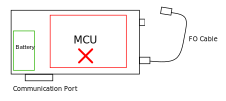
\includegraphics[width = 0.25 \textwidth]{"Pictures/Seal_Opened.png"}
            \caption{Seal Opened}
        \end{figure}
        
      \subsection{Problems}
        \begin{center}
            \begin{itemize}
                \item \textbf{Physical Tampering:} \\
                        If a state or other entity seeks to divert nuclear material, they could try to modify the seal, such it doesn't detect a disconnection of the optical fibre. Also temporary disabling of the device or storage medium could be a possibility.
                
                \item \textbf{Electronic Tampering:} \\
                    To ensure the authenticity of the logged events, they have to be \textbf{electronically signed}. If the confidential signing/encryption keys can be extracted or reversed from the device, entries can be inserted, deleted or modified at will.
                    
                \item \textbf{Radiation:} \\
                        High energy Radiation is known to corrupt memory or behaviour of a microcontroller. Therefore the device has to be protected against the radiation of the controlled material. Under no circumstances
                        should the radiation generate a false positive signature in the seal.
                        
                \item \textbf{Battery Life:} \\
                        As nuclear material can sit around many years, the sheal should have an andequately long Battery life. Continuous monitoring of the state of the fiber uses this scarce energy so the device \textbf{must}
                        be a low-power design.
                        
            \end{itemize}
        \end{center}
        
    \subsection{Solutions}
    \begin{center}
        \begin{itemize}
            \item \textbf{Physical Tampering}\\
                Using intrusion-detection switches the seal can monitor the integrity of its own enclosure. Attacks on the fiber can be mitigated by randomly pulsing the optical source and closely monitoring the time required for the light to be registred at the reciever.
                
            \item \textbf{Electronic Tampering}\\
                The encryption keys can be set at the factory and kept only in volatile memory, so they are destroyed if tampering with the device or the battery is detected.
                
                
        \end{itemize}
        
    \end{center}
\end{document}
